\documentclass{beamer}

\usetheme{Antibes}
\usecolortheme{seagull}

\usepackage{graphicx}
\usepackage{tikz}
\usepackage{listings}
\usepackage{colortbl}
\usepackage{color}

\tikzstyle{block} = [rectangle, draw, text width=4.5em, text centered, minimum height=2em]
\lstset{basicstyle=\small\ttfamily}

\lstset{
  language=Java,
  basicstyle=\ttfamily\small,
  keywordstyle=\color{blue},
  commentstyle=\color{green!60!black},
  stringstyle=\color{red},
  showstringspaces=false,
  breaklines=true
}

\definecolor{mygray}{rgb}{0.5,0.5,0.5}
\definecolor{mygreen}{rgb}{0,0.6,0}
\definecolor{myblue}{rgb}{0,0,0.8}
\lstset{language=XML,
        morekeywords={m:GetPrice, m:StockName},
        basicstyle=\ttfamily,
        keywordstyle=\color{myblue},
        commentstyle=\color{mygreen},
        stringstyle=\color{myblue},
        numbers=left,
        numberstyle=\tiny\color{mygray},
        stepnumber=1,
        numbersep=3pt,
        backgroundcolor=\color{white},
        tabsize=1,
        showspaces=false,
        showstringspaces=false
}

% Define Protobuf language
\lstdefinelanguage{protobuf}{
  keywords={message, optional, repeated, required, returns,
  service, rpc, package, syntax, string, int32, bool},
  keywordstyle=\color{blue}\bfseries,
  ndkeywords={bool, int32, float, double, string},
  ndkeywordstyle=\color{darkgray}\bfseries,
  identifierstyle=\color{black},
  tabsize=1,
  sensitive=false,
  comment=[l]{//},
  morecomment=[s]{/*}{*/},
  commentstyle=\color{purple}\ttfamily,
  stringstyle=\color{red}\ttfamily,
  morestring=[b]",
  morestring=[b]',
}

\definecolor{codegray}{gray}{0.9}
\newcommand{\code}[1]{\colorbox{codegray}{\texttt{#1}}}

\setbeamertemplate{navigation symbols}{} % Remove navigation symbols

\title{Programming Paradigms \& Practices}
\author{Mohamed Sweelam}
\institute{Software Engineer}
\date{}

% Add the title graphic here
%\titlegraphic{\includegraphics[width=7cm, height=3.5cm]{img/course-logo.png}}
\logo{
\includegraphics[height=1cm]{img/channel-logo-circular.png}}

\begin{document}

\begin{frame}
  \titlepage
\end{frame}

\begin{frame}{Outline}
  \tableofcontents
\end{frame}

\section{Course Objectives}
\begin{frame}
	\frametitle{Course Objectives}
		\begin{enumerate}
			\item<1-> Provide good Arabic content for the topic
			\item<2-> Provide comprehensive insights into programming paradigms
			\item<3-> Explore advanced programming techniques
			\item<4-> Discuss best practices for project structure and code quality
			\item<5-> Overview of deployment models and strategies
		\end{enumerate}
\end{frame}

\section{Understanding Programming Paradigms}
\begin{frame}{Understanding Programming Paradigms}
	\scriptsize
	\begin{block}{Definition \tiny{\textit{wikipedia}}}
		Programming paradigms are fundamental styles or approaches to computer programming, offering distinct methodologies for designing and structuring software.
	\end{block}
	
	\begin{block}{Importance \tiny{\textit{ChatGPT}}}
		Understanding different programming paradigms is crucial for selecting the right approach to solve specific problems, leading to more efficient and maintainable code.
	\end{block}
	
	\begin{alertblock}{Historical Context \tiny{\textit{wikipedia}}}
		Programming paradigms have evolved over time, with significant contributions from various programming languages that introduced unique features and concepts, shaping the way we write software today.
	\end{alertblock}
  
\end{frame}


\begin{frame}{Programming Paradigms Types}
	\small
	\begin{columns}[T] % The [T] option aligns the columns' content at the top
    	\begin{column}{.5\textwidth} % Left column and width
		\begin{itemize}
			\item Imperative Programming
			\item Procedural Programming
			\item Object-Oriented Programming
			\item Declarative Programming
			\item Functional Programming
			\item Event-Driven Programming
			\item Aspect-Oriented Programming
			\item Reactive Programming
		\end{itemize}
    	\end{column}
    	\begin{column}{.5\textwidth} % Right column and width
    		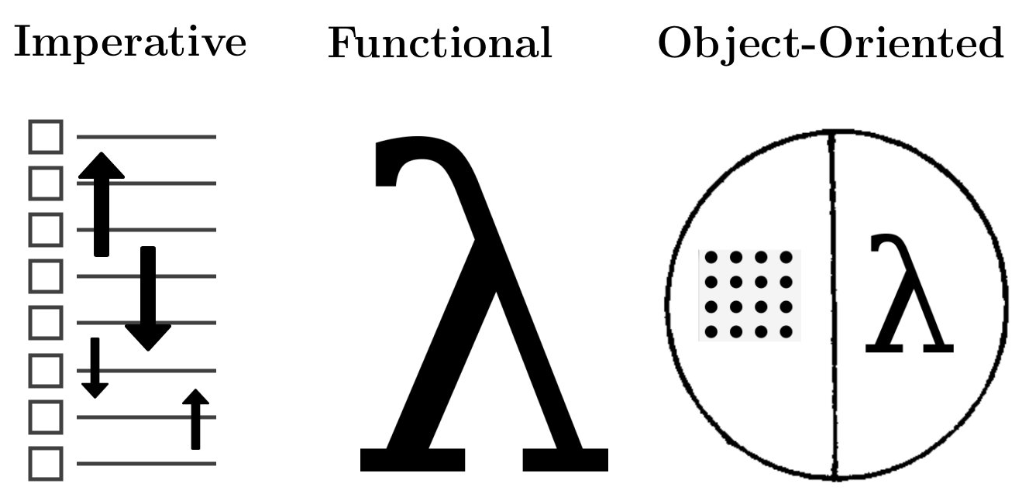
\includegraphics[width=0.99\textwidth, height=0.4\textheight]{img/para-types.png}
   		\end{column}
  	\end{columns}
\end{frame}

\begin{frame}[t]{Imperative Programming}
	\scriptsize
	\begin{itemize}
		\item<1-> In this paradigm, the program is a sequence of instructions that explicitly change the program state. It focuses on how to achieve a task.
		\item<2-> C, Python, Java (most common imperative languages have procedural features as well)
		\item<3-> \textbf{Key Concepts:} Variables, controls (loops,conditionals), and subroutines.
		\item<4->[]
			\begin{center}
				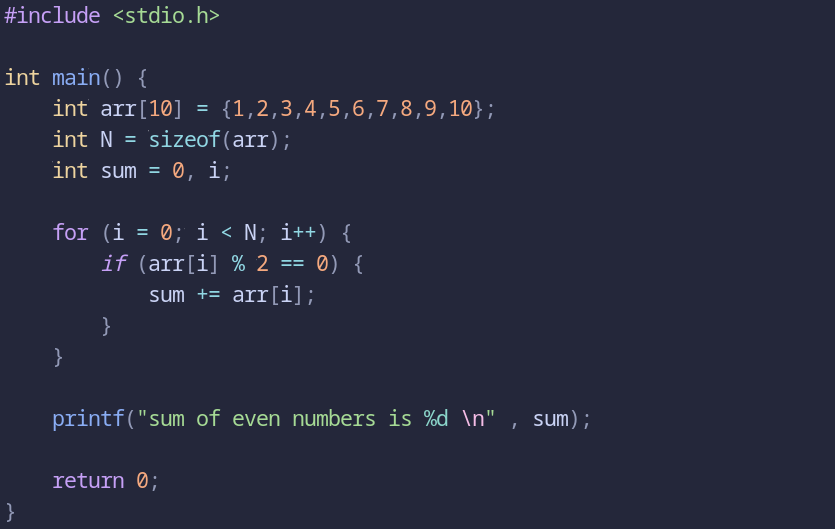
\includegraphics[width=0.6\textwidth, height=0.5\textheight]{img/c-example.png}
			\end{center}
	\end{itemize}
\end{frame}


\begin{frame}{Procedural Programming}
	\scriptsize
	\begin{itemize}
		\item<1-> A subset of imperative programming that structures programs as a series of procedures or functions. These procedures perform operations on data and are reusable.
		\item<2-> C, Pascal, Python.
		\item<3-> \textbf{Key Concepts:} Procedures, functions, modular programming.
		\item<4->[]
			\begin{center}
				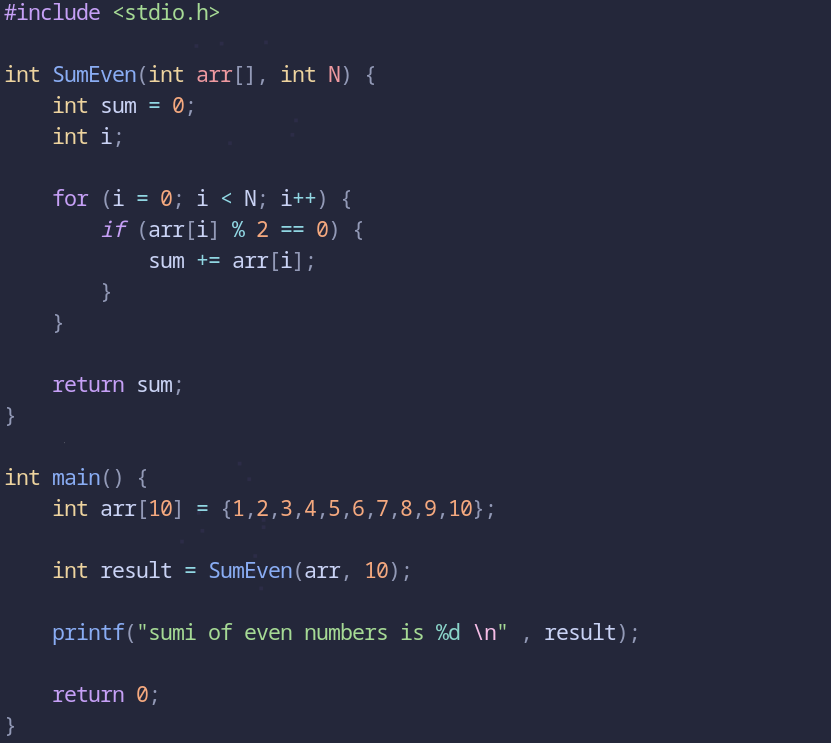
\includegraphics[width=0.6\textwidth, height=0.5\textheight]{img/c-even-sum.png}
			\end{center}
	\end{itemize}
\end{frame}


\begin{frame}{Object-Oriented Programming}
	\scriptsize
	\begin{itemize}
		\item<1-> Focuses on designing software using objects that represent real-world entities. Objects are instances of classes that encapsulate data and behavior.
		\item<2-> Java, C\#, PHP, Ruby.
		\item<3-> \textbf{Key Concepts:}  Classes, objects, polymorphism, encapsulation, abstraction.
		\item<4-> \textit{let's try an example}
	\end{itemize}
\end{frame}

\begin{frame}[t]{Declarative Programming}
	\scriptsize
	\begin{itemize}
		\item<1-> In this paradigm, the programmer specifies what the program should accomplish, rather than how to accomplish it. This is often used in conjunction with other paradigms like logical or functional programming.
		\item<2-> SQL, HTML, CSS.
		\item<3-> \textbf{Key Concepts:} Expressions, constraints, high-level abstraction.
		\item<4->[]
			\vspace{4mm}
			\begin{center}
				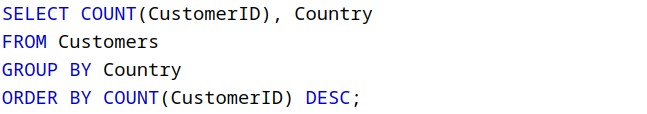
\includegraphics[width=0.6\textwidth, height=0.2\textheight]{img/sql-example.png}
			\end{center}
	\end{itemize}
\end{frame}

\begin{frame}[t]{Functional Programming}
	\scriptsize
	\begin{itemize}
		\item<1-> Emphasizes computation using mathematical functions and avoids changing states or mutable data. Functions are first-class citizens and can be passed as arguments and returned as values.
		\item<2-> Haskell, Lisp, Scala, Erlang, F\#.
		\item<3-> \textbf{Key Concepts:} Pure functions, immutability, higher-order functions, recursion.
		\item<4->[]
			\vspace{1mm}
			\begin{center}
				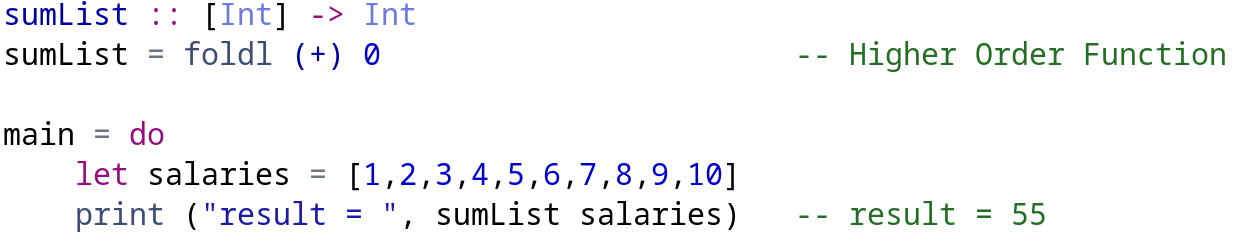
\includegraphics[width=0.7\textwidth, height=0.17\textheight]{img/hashkel-salary-sum.png}
			\end{center}
	\end{itemize}
\end{frame}



\begin{frame}[t]{Functional Programming}
	\begin{itemize}
		\item[]
			\begin{center}
				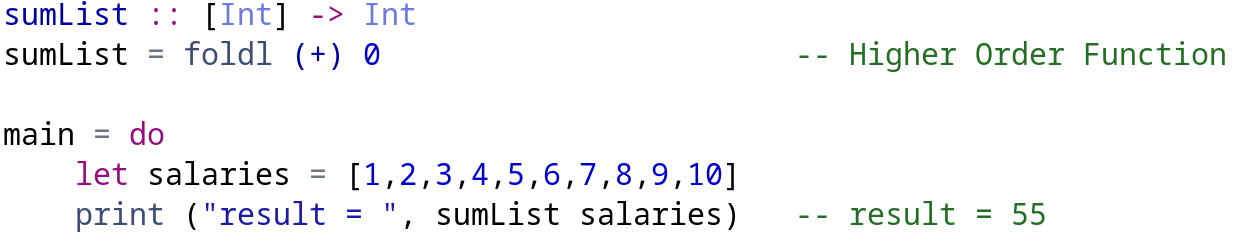
\includegraphics[width=0.7\textwidth, height=0.25\textheight]{img/hashkel-salary-sum.png}
			\end{center}
		\item<2->[]
			---------------------------------------------------------------------------
			\begin{center}
				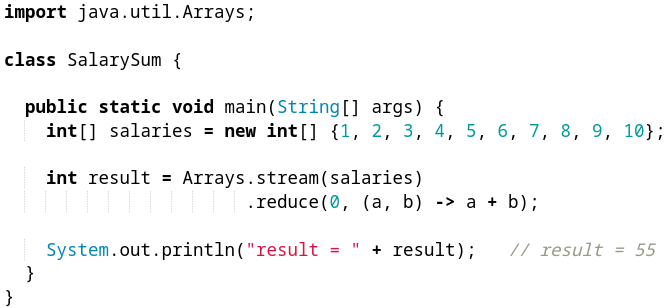
\includegraphics[width=0.7\textwidth, height=0.4\textheight]{img/java-sum-list.png}
			\end{center}

			
	\end{itemize}
\end{frame}



\section{Advanced Programming Techniques}
\begin{frame}{Advanced Programming Techniques}
	\scriptsize
	\begin{itemize}
		\item<1-> Multithreading and Concurrency
		\item<2-> Reactive Programming and Asynchronous Streams
		\item<3-> Memory Management and Optimization
		\item<4-> Effective Error Handling and Debugging
	\end{itemize}
	\begin{center}
		% \includegraphics[width=0.6\textwidth, height=0.4\textheight]{img/advanced-techniques.png}
	\end{center}
\end{frame}

\section{Project Structure and Code Quality}
\begin{frame}{Project Structure and Code Quality}
	\begin{itemize}
		\item Organizing Your Codebase
		\item Implementing Best Practices for Readability and Maintainability
		\item Writing Clean and Testable Code
		\item Integrating Continuous Integration and Automated Testing
	\end{itemize}
\end{frame}

\section{Deployment Models}
\begin{frame}{Deployment Models}
	\begin{itemize}
		\item Understanding Different Deployment Strategies
		\item Containerization and Orchestration with Docker and Kubernetes
		\item Continuous Deployment and Delivery Pipelines
		\item Monitoring and Maintaining Production Environments
	\end{itemize}
\end{frame}

\section{Conclusion}
\begin{frame}{Conclusion}
	\begin{itemize}
		\item Recap of Key Learnings
		\item Emerging Trends in Software Development
	\end{itemize}
\end{frame}

\end{document}
